\section{The centrifugal pump}
\label{sec:pumps:inside}


\subsection{Pump types}

\begin{figure}[!h]
  \centering{
    \begin{subfigure}{0.8\textwidth}
      \includegraphics[height=\textwidth,angle=-90]{pumps/centrifugalPump_diffuser.png}
      \caption{Pump with outlet diffuser. Reproduced from
        \cite{LeonardULg}.}
    \end{subfigure}
    \begin{subfigure}{0.7\textwidth}
      \includegraphics[width=\textwidth]{pumps/centrifugalPump_igv.png}
      \caption{Pump with inlet guide vane. Reproduced from \cite{TZC+96}.}
    \end{subfigure}
  }
  \caption{Centrifugal pump}
  \label{fig:centrifugalPump}
\end{figure}
The pump consists of the following parts, encountered successively:
\begin{itemize}
\item the \emph{distributor}, potentially equipped with \emph{inlet
    guide vanes (IGV)}, is responsible of guiding the flow from the
  suction pipe (I) to the impeller, and distributing the flow
  tangentially homogeneously over the \emph{eye} of the
  \emph{impeller};
\item as the sole rotating part of the pump the \emph{impeller} is
  responsible for converting power from the shaft to the mechanical
  energy / total head of the flow, as it passes from the eye (1)
  towards the outlet (2);
\item at the outlet of the impeller, sometimes a \emph{diffusor} is
  foreseen, potentially equipped with vanes, which converts part of
  the kinetic energy / dynamic head available at the impeller outlet
  (2) to pressure / manometric head at station (2$^\prime$);
\item Finally the \emph{volute} collects the flow from the
  circumference of the diffuser thereby ideally maintaining
  circumferential uniformity of the flow. At the end of the volute,
  often a conical diffusor is found.
\end{itemize}


\section{Head balance}
\label{sec:pumps:head}

In the following sections, we will look into the evolution of the head
as the flow progresses through the pump at a given operation point.
\begin{figure}[!h]
  \centering{\tikzsetnextfilename{headDiagramPump}
\begin{tikzpicture}
  
  \scriptsize
  
  %%% pump inlet
  \def\hI{40}  
  \def\vI{10}

  %%% losses inlet --> impeller eye
  \def\lIe{10}

  %%% impeller eye
  \def\ve{20}   
  \def\he{\hI-\lIe}
  
  %%% impeller performance
  \def\hi{140}  %%% indicated head
  \def\li{10}   %%% impeller losses
  
  %%% impeller outer rim
  \def\vr{60}          
  \def\hr{\he+\hi-\li}
  
  %%% losses in diffuser
  \def\lrd{15} 
  
  %%% diffuser outlet
  \def\vd{15}       
  \def\hd{\hr-\lrd}
  
  %%% volute losses
  \def\ldO{10}
  
  %%% outlet
  \def\vO{10}
  \def\hO{\hd-\ldO}
  
  \begin{axis}[
    width = \textwidth,
    height =0.4\textheight,
    xtick = data,
    xticklabels = {Inlet,Impeller eye,Impeller outlet,Volute inlet,Outlet},
    ytick = \empty,
    axis lines = center,
    xmin = 0,
    xmax = 6,
    ymin = 0,
    ymax = 170,
    % xlabel = $station$,
    % ylabel = $\head$,
    legend style   = {draw=none,anchor=west,at={(0.05,0.5)}},
    legend entries = {total head,static head},
    >=latex
    ],
    \addplot [black,line width=1.5pt] coordinates {
      (0.5,\hI) 
      (1.5,\he) 
      (2.5,\hr) 
      (3.5,\hd) 
      (4.5,\hO)};
    \addplot [dashed,line width=1.5pt] coordinates {
      (0.5,\hI-\vI) 
      (1.5,\he-\ve)
      (2.5,\hr-\vr) 
      (3.5,\hd-\vd) 
      (4.5,\hO-\vO)};
    
    \addplot [dashed] coordinates {(0.5,0) (0.5,\hI)};
    \addplot [dashed] coordinates {(1.5,0) (1.5,\he)};
    \addplot [dashed] coordinates {(2.5,0) (2.5,\hr)};
    \addplot [dashed] coordinates {(3.5,0) (3.5,\hd)};
    \addplot [dashed] coordinates {(4.5,0) (4.5,\hO)};
    
    \addplot [dashed] coordinates {(0,\hI) (5,\hI)}
    node [pos=0.03,left,above]{$\head_i$};
    \addplot [dashed] coordinates {(0,\hO) (5,\hO)}
    node [pos=0.03,left,above]{$\head_o$};
    
    \addplot [dashed] coordinates {(0,\he) (5.6,\he)};
    \addplot [dashed] coordinates {(0,\hr) (5.6,\hr)};
    
    \addplot [<->,>=latex] 
    coordinates {(5.4,\he) (5.4,\hr)} 
    node [midway,right] {$\dhead_t - \loss_{12}$};
    \addplot [<->,>=latex] 
    coordinates {(4.8,\hI) (4.8,\hO)} 
    node [midway,right] {$\dhead_p$};
    \addplot [<->,>=latex] 
    coordinates {(4.8,\hr) (4.8,\hO)} 
    node [midway,right] {$\loss_{2o}$};
    \addplot [<->,>=latex] 
    coordinates {(4.8,\he) (4.8,\hI)} 
    node [midway,right] {$\loss_{i1}$};
    
  \end{axis}

\end{tikzpicture}}
  \caption{Head diagram for the flow in the pump}
  \label{fig:headDiagramPump}
\end{figure}

The vanes or blades are responsible for guiding the flow in the stator
resp. rotor parts. In theory, one would need an infinite number of
zero-thickness blades to ensure the same flow path to all fluid
particles. We will make this hypothesis for the time being, and
correct for the effects due to the finite number of blades later on.
We furthermore assume that the pump is in a stabilised working
condition and that therefore the average velocity of the flow
particles in any point in the machine is constant in time.

\subsection{Indicated head}

At station 1, corresponding to the inlet of the impeller, the absolute
flow angle $\alpha_1$ is imposed by the inlet distributor. We can then
determinate the flow triangle from the impeller flow rate $\vFlow_i$:
\begin{align*}
  \aVel_{m,1} &= \frac{\vFlow_i}{2 \pi R_1 h_1 (1-b_1)} &
  \aVel_{u,1} &= \aVel_{m,1}~\tan(\alpha_1) &
  \rVel_{u,1} &= \aVel_{u,1} - \fVel_1 = \aVel_{u,1} - \rot R_1
\end{align*}
whereby the rotation velocity $\fVel_1 = \rot R_1$. At station 2,
corresponding to the outlet of the impeller, the relative flow angle
$\beta_2$ is fixed by the rotating blades. Therefore, we can compute
the velocity triangle by
\begin{align*}
  \aVel_{m,2} &= \frac{\vFlow_i}{2 \pi R_2 h_2 (1-b_2)} &
  \rVel_{u,2} &= \aVel_{m,2}~\tan(\beta_2) &
  \aVel_{u,2} &= \rVel_{u,2} + \fVel_2 = \rVel_{u,2} + \rot R_2
\end{align*}
The \emph{indicated power} $\power_i$ corresponds to the total
hydraulic power conveyed by the impeller to the fluid. Following
Euler's equation, this power is given by
\begin{align*}
  \power_i = \dens \vFlow_i \left(\fVel_2 \aVel_{u,2} - \fVel_1 \aVel_{u,1}\right)
\end{align*}
The corresponding \emph{indicated} or \emph{theoretical head}
$\dhead_i$ is then given by
\begin{align*}
  \dhead_i &= \frac{\power_i}{\dens \vFlow_i g} 
  = \frac{\fVel_2 \aVel_{u,2} - \fVel_1 \aVel_{u,1}}{g} 
  = 
  \frac{\aVel_2^2 - \aVel_1^2}{2g} - 
  \frac{\rVel_2^2 - \rVel_1^2}{2g} + 
  \frac{\fVel_2^2 - \fVel_1^2}{2g}
\end{align*}
$\dhead_i$ corresponds to the enthalpy increase of the flow, or
equivalently to the increase in head if no losses were incurred. The
conservation of mechanical energy between stations 1 and 2 on the
other hand then gives us
\begin{align*}
  \frac{\pres_2 - \pres_1}{\dens \grav} + 
  \frac{\aVel_2^2 -  \aVel_1^2}{2\grav} + 
  z_2 - z_1 + \loss_{12} = \dhead_i
\end{align*}
Combining both expressions, we find
\begin{align*}
  \frac{\pres_2 - \pres_1}{\dens \grav} + z_2 - z_1 + \loss_{12} =
  \frac{\fVel_2^2 - \fVel_1^2}{2g} - \frac{\rVel_2^2 - \rVel_1^2}{2g}
\end{align*}
showing that the increase in pressure and elevation results from the
Coriolis forces in the impeller, as well as the diffusion of the
relative velocity.

%% -----------------------------------------------------------------------------
\subsection{Hydrodynamic losses}
\label{subsec:pumps:hydrodynamicLosses}
%% -----------------------------------------------------------------------------

Head losses are irreversibilities occuring all along the flow
path. They include hydrodynamic and separation losses and reduce the
part of the hydraulic power that is converted into mechanical energy.

\subsubsection{Distributed losses}

Distributed losses result first of all from the friction on the walls
of the distributor, the impeller, the diffuser and the volute. These
losses are approximately proportional to the square of the velocity
and therefore to the dynamic head. The friction coefficients are
function of the local Reynolds number and the roughness of the walls.

Due to the finite number of blades, high blade loading etc. the flow
will not follow the ideal flow path and may even separate in the
smooth flow passages due to accumulation of boundary layers. This
so-called secondary flows leads to important additional losses, which
can change rapidly with the flow conditions. Consequently the
prediction of distributed losses typically requires detailed CFD
computations, particularly when operating at off-design conditions.

\todo{Flow pattern in rotor passages}

\subsubsection{Incidence losses} 

\begin{wrapfigure}{R}{0.3\textwidth}
  \centering{
    \includegraphics[width=0.3\textwidth]{pumps/shockLosses.png}}
  \caption{Incidence losses}
  \label{fig:shockIncidence}
\end{wrapfigure}
Incidence losses result from misalignment of the flow with the leading
edge of blades, occuring at inlet guide vanes, the impeller blades,
diffusor vanes and volute tongue. The historic denomination
\emph{shock losses} is unfortunate, not only because actual shocks
only occur in compressible flows, but also since the actual loss does
not orginate from discontinuities, but from the very rapid diffusion
of the stream tubes, after the blockage induced by the leading edge
separation as shown in figure \ref{fig:shockIncidence}. In a correctly
designed machine, incidence losses only occur at off-design
conditions.
\begin{figure}[!h]
  \centering{
\tikzsetnextfilename{shockLosses}
\begin{tikzpicture}[scale=0.8]

  %\scriptsize

  \def\a{30}
  
  \def\vrNom{6}
  \def\wrNom{\vrNom}
  \def\vrAct{4}
  \def\wrAct{\vrAct}
  \def\uTan{12}
  
  \def\vuNom{\vrNom*tan(\a)}
  \def\vuAct{\vrAct*tan(\a)}
  
  \def\bNom{atan((\uTan-\vuNom)/\vrNom)}
  \def\bAct{atan((\uTan-\vuAct)/\vrAct)}
  

  \coordinate(CNom) at (0,0); %% top
  \coordinate(BNom) at ({\vuNom-\uTan},-\wrNom);       %% 
  \coordinate(ANom) at ({\vuNom},-\wrNom);
  \coordinate(DNom) at (0,-\wrNom);
  
  \draw[<->,>=latex,line width=1.5pt] 
  (BNom) node [left] {$B$} --
  (CNom) node [pos=0.1,left,above,sloped]{$\rVelV$} node [at end,above] {$C$} --
  (DNom) node [pos=0.9,left]{$\rVel_m$}
  pic["$\beta$", draw=black,color=black,<-, angle eccentricity=1.4, angle radius=1.6cm]
  {angle=BNom--CNom--DNom};

  \draw[->,>=latex,line width=1.5pt] 
  (DNom) --
  (CNom) node [pos=0.1,right]{$\aVel_m$}  --
  (ANom) node [pos=0.9,right,above,sloped]{$\aVelV$} node [at end,right]{$A$}
  pic["$\alpha$", draw=black,color=black,->, angle eccentricity=1.4, angle radius=1.4cm]
  {angle=DNom--CNom--ANom};

  \coordinate(BAct) at ({\vuAct-\uTan},-\wrAct);       %% 
  \coordinate(BShock) at ({-\vrAct*tan(\bNom)},-\wrAct);
  
  \coordinate(BActp) at ({\vuAct-\uTan},0);       %% 
  \coordinate(BShockp) at ({-\vrAct*tan(\bNom)},0);
  
  
  \coordinate(BActpp) at ({\vuAct-\uTan},{-0.05*\vrNom});       %% 
  \coordinate(BShockpp) at ({-\vrAct*tan(\bNom)},{-0.05*\vrNom});
  

  \coordinate(AAct) at ({\vuAct},-\wrAct);
  \coordinate(DAct) at (0,-\wrAct);
  
  \draw[<->,>=latex,color=red,line width=1.5pt] 
  (BAct) node [left] {$B^\prime$} --
  (CNom) node [pos=0.2,above,sloped]{$\rVelV^\prime$}  --
  (DAct) node [pos=0.8,left]{$\rVel_m^\prime$}
  pic["$\beta^\prime$", draw=red,color=red,<-, angle eccentricity=1.4, angle radius=0.8cm]
  {angle=BAct--CNom--DAct};

  \draw[->,>=latex,line width=1.5pt,color=red] 
  (DAct) --
  (CNom) node [pos=0.2,right]{$\aVel_m^\prime$}  --
  (AAct) node [pos=0.8,right,above,sloped]{$\aVelV^\prime$} node [at end,right]{$A^\prime$};


  \draw[->,>=latex,line width=1.5pt] 
  (BNom) --(ANom) node [midway,above]{$\fVelV$};
  \draw[->,>=latex,line width=1.5pt,color=red] 
  (BAct) --(AAct) node [midway,above]{$\fVelV$};
  \draw[dotted,line width=1pt] (BAct) -- (BNom){};
  \draw[] (BShock) node [below]{$B^{\prime\prime}$};
  
  \draw[dotted,line width=1pt] (BAct) -- (BActp){};
  \draw[dotted,line width=1pt] (BShock) -- (BShockp){};
  \draw[->,line width=1.5pt] (BActpp) -- node[midway,above]{$\rVelV_s$} (BShockpp) {};

  
  \draw[->,>=latex,color=blue,line width=1.5pt] 
  (CNom) --
  (BShock) node [pos=0.8,sloped,above,color=blue]{$\rVelV^{\prime\prime}$};

  
\end{tikzpicture}
}
  \caption{Computation of the shock velocity $\rVel_s$}
  \label{fig:shockLosses}
\end{figure}
The estimation of the shock losses hinges on the definition of the
\emph{shock velocity} $\vel_s$, which corresponds to the tangential
deviation required to align the flow with the blade. The shock loss is
assumed to be of the form
\begin{align*}
  \loss_{s} = k_s \frac{\vel_s^2}{2 \grav}
\end{align*}
with the loss coefficient $k_s = 0.5 \ldots 0.9$. 

Take for instance the eye of the impeller, for which we illustrated
the velocity triangles in figure \ref{fig:shockLosses}. In the
velocity triangle $\widehat{BCA}$, corresponding to the nominal flow
rate $\vFlow$, the flow is fully aligned with the blade, \ie the
relative flow angle $\beta$ corresponds to the blade flow angle. Now
we construct the velocity triangle at the lower flow rate
$\vFlow^\prime$:
\begin{itemize}
\item Assuming that the inlet guide vane setting is not changed, the
  absolute flow angle $\alpha$ is the same for both conditions;
\item obviously also the rotor velocity $\fVelV$ is the same. 
\item the meridional velocity $\aVel_m^\prime$ has changed
  proportionally to the flow rate:
  \begin{align*}
    \frac{\aVel_m}{\aVel_m^\prime} = 
    \frac{\rVel_m}{\rVel_m^\prime} = 
    \frac{\vFlow}{\vFlow^\prime}
  \end{align*} 
\end{itemize}
Therefore, the velocity triangle has changed to $\widehat{B^\prime C
  A^\prime}$; one sees that the relative flow angle is now
$\beta^\prime$.
Now we compute the change required to align the flow with the blade
and therefore force the relative flow angle to $\beta$. Since the flow
rate should remain the same, the meridional velocity $\rVel_m^\prime$
can not change. Therefore only the tangential velocity
$\rVel_u^\prime$ is changed to $\rVel_u^{\prime\prime}=\rVel_u^\prime
- \rVel_s$. The resulting velocity triangle $\widehat{B^{\prime\prime}
  C A^\prime}$ is geometrically similar to the nominal velocity
triangle $\widehat{BCA}$. Therefore:
\begin{align*}
  \frac{\fVel}{\fVel - \rVel_s} = \frac{\rVel_m}{\rVel_m^\prime} = \frac{\vFlow}{\vFlow^\prime}
\end{align*}
Hence the shock loss is found to be:
\begin{align*}
  \loss_s = k_s \frac{\fVel^2}{2\grav}~\left(1 - \frac{\vFlow^\prime}{\vFlow}\right)^2
\end{align*}

One could theoretically avoid the shock losses by changing the inlet
guide vane setting to provide an absolute flow angle $\alpha^\prime$
as seen in figure \ref{fig:prewhirl}.
\begin{figure}[!h]
  \centering{
    \tikzsetnextfilename{prewhirl}
\begin{tikzpicture}[scale=0.8]

  %\scriptsize

  \def\a{30}
  
  \def\vrNom{6}
  \def\wrNom{\vrNom}
  \def\vrAct{4}
  \def\wrAct{\vrAct}
  \def\uTan{12}
  
  \def\vuNom{\vrNom*tan(\a)}
  \def\vuAct{\vrAct*tan(\a)}
  
  \def\bNom{atan((\uTan-\vuNom)/\vrNom)}
  \def\bAct{atan((\uTan-\vuAct)/\vrAct)}
  

  \coordinate(CNom) at (0,0); %% top
  \coordinate(BNom) at ({\vuNom-\uTan},-\wrNom);       %% 
  \coordinate(ANom) at ({\vuNom},-\wrNom);
  \coordinate(DNom) at (0,-\wrNom);
  
  \draw[<->,>=latex,line width=1.5pt] 
  (BNom) node [left] {$B$} --
  (CNom) node [pos=0.1,left,above]{$\rVelV$} node [at end,above] {$C$} --
  (DNom) node [pos=0.9,left]{$\rVel_m$}
  pic["$\beta$", draw=black,color=black,<-, angle eccentricity=1.4, angle radius=1.4cm]
  {angle=BNom--CNom--DNom};

  \draw[->,>=latex,line width=1.5pt] 
  (DNom) --
  (CNom) node [pos=0.1,right]{$\aVel_m$}  --
  (ANom) node [pos=0.9,right,above]{$\aVelV$} node [at end,right]{$A$}
  pic["$\alpha$", draw=black,color=black,->, angle eccentricity=1.4, angle radius=1.6cm]
  {angle=DNom--CNom--ANom};

  \coordinate(BAct) at  ({-\vrAct*tan(\bNom)},-\wrAct);
  \coordinate(BActp) at ({-\vrAct*tan(\bNom)},0);
  
  \coordinate(AAct) at ({-\vrAct*tan(\bNom)+\uTan},-\wrAct);
  \coordinate(DAct) at (0,-\wrAct);
  
  \draw[<->,>=latex,color=red,line width=1.5pt] 
  (BAct) node [left] {$B^\prime$} --
  (CNom) node [pos=0.2,left,above]{$\rVelV^\prime$}  --
  (DAct) node [pos=0.8,left]{$\rVel_m^\prime$};

  \draw[->,>=latex,line width=1.5pt,color=red] 
  (DAct) --
  (CNom) node [pos=0.2,right]{$\aVel_m^\prime$}  --
  (AAct) node [pos=0.8,right,above]{$\aVelV^\prime$} node [at end,right]{$A^\prime$}
  pic["$\alpha^\prime$", draw=red,color=red,->, angle eccentricity=1.4, angle radius=0.8cm]
  {angle=DAct--CNom--AAct};


  \draw[->,>=latex,line width=1.5pt] 
  (BNom) --(ANom) node [midway,above]{$\fVelV$};
  \draw[->,>=latex,line width=1.5pt,color=red] 
  (BAct) --(AAct) ;
  \draw[dotted,line width=1pt] (AAct) -- (ANom){};
  
\end{tikzpicture}

  }
  \caption{Avoiding shock losses using prewhirl}
  \label{fig:prewhirl}
\end{figure}



%%% Local Variables: 
%%% mode: latex
%%% TeX-master: "../MECA0467"
%%% End: 
